\chapter{Introducción}
\pagenumbering{arabic}

La huella digital es la recopilación sistemática sobre un determinado dispositivo con la finalidad de identificarlo, singularizarlo y perfilarlo. Este conjunto de datos permite prácticamente, de forma unívoca, identificar dicho terminal y en cuestión a la persona o grupo de personas que puedan estar usándolo. Por lo general, los terminales como los teléfonos móviles, tabletas, portátiles y ordenadores de sobremesa, son usados por una sola persona y por ello, podemos asumir que los datos recopilados de cierto dispositivo pertenecen a una persona en concreto.\par

Actualmente, las aplicaciones web prestan servicios de forma totalmente gratuita a cambio de los datos que recopilan de los usuarios. En la mayoría de casos esta información se rentabiliza a través de servicios de marketing y publicidad que desean vender un producto o servicio determinado. Por ello, estos servicios necesitan perfilar al usuario en cuestión para así ofrecerle un producto que les pueda interesar. Las entidades usan estos mecanismos de recopilación de datos con todos los terminales que se conecten a sus servidores, para así poder hacer un seguimiento del usuario y elaborar un perfil.\par

La técnica de seguimiento más conocida  son las \textit{cookies}, las cuales se almacenan en el propio dispositivo y que luego son usadas para estudiar la estadística de uso de la aplicación web y para mejorar la experiencia del usuario. Es común encontrar cláusulas de privacidad que permiten al usuario dar o no su consentimiento para el uso de éstas. Algunos exploradores ofrecen la posibilidad de deshabilitar su uso y ciertos antivirus realizan borrados periódicos de los ficheros de rastreo, pero la mayoría de aplicaciones web no dejan acceder a sus servicios, o la totalidad de los mismos, si el usuario no permite su uso. El uso de las técnicas de huella digital permite que, en el caso de que las \textit{cookies} sean eliminadas, no se pierda la trazabilidad sobre el usuario. Tecnologías como JavaScript, Flash y Microsoft Silverlight, facilitan la implementación de métodos para recoger información muy concreta del dispositivo, como es el tamaño de la pantalla o la versión del sistema operativo. La combinación de estas características permite perfilar al usuario e identificarlo.  \par

\section{Objetivos}
 
El principal objetivo de este proyecto es crear una aplicación web que permita recopilar los datos de un terminal, aplicando las distintas técnicas de \textit{fingerprinting}, y elaborar un perfil en base a ellos. En concreto tenemos las siguientes metas:
\begin{itemize}
    \item Crear una aplicación escalable, para que en el futuro se pueda continuar desarrollando según se requiera.
    \item Investigar la variedad de métodos de huella digital e implementarlos.
    \item Almacenar la información recogida, de la cual se hará un perfilado y se guardará en una base de datos.
\end{itemize}

\section{Plan de trabajo}
Para el desarrollo del proyecto se ha fijado una planificación de tal forma que se cubre las fases de investigación, análisis de requisitos, implementación, testing y la memoria.\par
En la figura~\ref{fig:diagramaGantt} se puede observar el \textit{diagrama de Gantt}. Tras la ampliación de los plazos de entrega, se actualizaron las tareas posteriores y sus respectivos tiempos. Las tareas desglosadas consisten en:
\begin{itemize}
    \item \textbf{Investigación}: Recogida de información acerca de las distintas técnicas existentes\cite{Huella} para obtener información de los dispositivos. Esto incluye ciertas páginas que determinan la huella digital del navegador\cite{amiunique}.
    \item \textbf{Análisis de requisitos}: Valoración sobre qué lenguajes de programación y herramientas vamos a usar para el desarrollo del proyecto.
    \item \textbf{Implementación}: Puesta en marcha del proyecto. En esta etapa del desarrollo se implementaría la aplicación web con su respectiva base de datos.
    \item \textbf{Pruebas}: Comprobación del funcionamiento de la aplicación y resolución de las posibles incidencias.
    \item \textbf{Memoria}: Elaboración de la memoria.
\end{itemize}
\begin{figure}[b]
    %\centering
    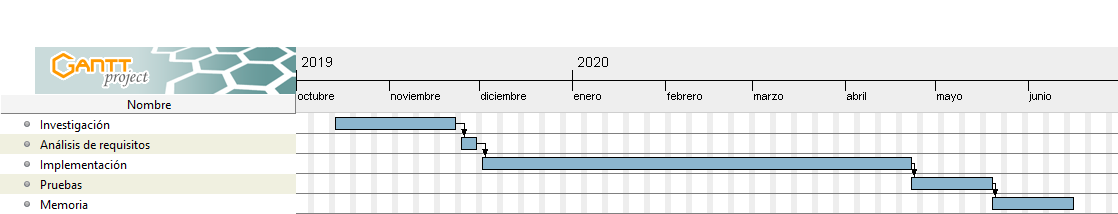
\includegraphics[width=1\textwidth, height=4cm]{Images/diagramaGantt.png}
    \caption{diagrama de Gantt}
    \label{fig:diagramaGantt}
\end{figure}